\setchapterstyle{kao}
\setchapterpreamble[u]{\margintoc}

\chapter{Search for an Excess of Heavy Neutral Lepton Events}
\labch{analysis}

The measurement performed in this thesis is the search for an excess of HNL events in the \SI{10}{years} of IceCube DeepCore data. In principle the two physics parameters to be probed are the mass of the HNL, $m_4$, and the mixing between the fourth heavy mass state and the SM $\tau$ sector, $|U_{\tau4}|^2$. Since the mass itself influences the production and decay kinematics of the event and the accessible decay modes, individual mass sets were produced as described in \refsec{model_specific_simulation}. The mass slightly influences the energy distribution, while the mixing both changes the overall scale of the HNL events and the shape in energy and PID. IceCube DeepCore is suited to measure the excess which appears around and below \SI{20}{\gev}, due to its production from the atmospheric tau neutrinos, although a reduced lower energy threshold could improve the analysis. The measurement will be performed for the three mass sets individually, while the mixing is the parameter that can be varied continuously and will be measured in the fit. 


\section{Final Level Sample} \labsec{analysis_samples}

The final level sample of this analysis always consists of the neutrino and muon MC introduced in \refsec{sm_event_generation} and one of the three HNL samples explained in \refsec{model_specific_simulation}. All of those simulation sets and the \SI{10}{years} of IceCube DeepCore data are processed through the full processing and event selection chain described in \refsec{processing_chain, reconstruction} leading to the final level sample. Since applying the last cuts from \refsec{analysis_cuts} leaves an insignificant amount of pure noise events in the sample, the noise simulation is not included in the analysis and won't be listed here.


\todo{add information about the matter profile used }
\todo{add information about the oscillation probability calculation and the software used for it}

\subsection{Expected Rates/Events}

The rates and the expected number of events for the SM background are shown in \reftab{background_final_level_expectation}. The explicit detector livetime in the \SI{10}{} years data taking period is \SI{9.28}{years}. The rates are calculated by summing the weights of all events in the final level sample, while the uncertainties are calculated by taking the square root of the sum of the weights squared. The expected number of events is calculated by multiplying the rate with the livetime. The individual fractions show that this sample is neutrino dominated where the majority of events are $\nu_\mu$-CC events.

\begin{table}
    \begin{tabular}{ lccc }
    \hline\hline
    \textbf{Type} & \textbf{Rate [\si{\milli\hertz}]} & \textbf{Events (in \SI{9.28}{years})} & \textbf{Fraction [\si{\percent}]} \\ 
    \hline\hline
    $\nu_\mu^\rm{CC}$   & 0.3531 & 103321 $\pm$ 113 & 58.9 \\
    $\nu_e^\rm{CC}$     & 0.1418 & 41490 $\pm$ 69 & 23.7 \\
    $\nu_\rm{NC}$       & 0.0666 & 19491 $\pm$ 47 & 11.1 \\
    $\nu_\tau^\rm{CC}$  & 0.0345 & 10094 $\pm$ 22 & 5.8 \\
    $\mu$               & 0.0032 & 936 $\pm$ 15 & 0.5 \\
    \hline
    total               & 0.5991 & 175336 $\pm$ 143 & 100.0  \\
    \hline
    \end{tabular}
\caption[Final level background event/rate expectation]{Final level rates and event expectation of the SM background particle types.}
\labtab{background_final_level_expectation}
\end{table}

\todo{Should I adapt the total numbers to match the sum of the rounded individual parts?}

\reftab{signal_final_level_expectation} shows the rates and expected number of events for the HNL signal simulation. The expectation depends on the mass and the mixing and shown here are two example mixings for all the three masses that are being tested in this work. A mixing of $0.0$ would result in no HNL events at all. It can already be seen that for the smaller mixing of $|U_{\tau4}|^2=10^{-3}$ the expected number of events is very low, while at the larger mixing of $|U_{\tau4}|^2=10^{-1}$ the number is comparable to the amount of muons in the background sample. 

\begin{table}[h]
    \begin{tabular}{ lcc }
    \hline\hline

    \textbf{HNL mass} & \textbf{Rate [\si{\micro\hertz}]} & \textbf{Events (in \SI{9.28}{years})} \\

    \hline\hline
    \textbf{$|U_{\tau4}|^2=10^{-1}$} & & \\ 
    \hline
    \SI{0.3}{\gev} & 3.3298 $\pm$ 0.0053 & 974.5 $\pm$ 1.6 \\
    \SI{0.6}{\gev} & 3.0583 $\pm$ 0.0058 & 895.0 $\pm$ 1.7 \\
    \SI{1.0}{\gev} & 2.4988 $\pm$ 0.0059 & 731.3 $\pm$ 1.7 \\
    \hline
    \textbf{$|U_{\tau4}|^2=10^{-3}$} & & \\ 
    \hline
    \SI{0.3}{\gev} & 0.0057 & 1.67 $\pm$ 0.01 \\
    \SI{0.6}{\gev} & 0.0220 & 6.44 $\pm$ 0.01 \\
    \SI{1.0}{\gev} & 0.0248 & 7.27 $\pm$ 0.01 \\
    % \SI{0.3}{\gev} & 0.00571 $\pm$ 0.00002 & 1.67 $\pm$ 0.01 \\
    % \SI{0.6}{\gev} & 0.02200 $\pm$ 0.00004 & 6.44 $\pm$ 0.01 \\
    % \SI{1.0}{\gev} & 0.02484 $\pm$ 0.00005 & 7.27 $\pm$ 0.01 \\
    \hline
    \end{tabular}
\caption[Final level signal event/rate expectation]{Final level rates and event expectations of the HNL signal for all three masses and two example mixing values.}
\labtab{signal_final_level_expectation}
\end{table}


\subsection{Analysis Binning}

The identical binning to the analysis performed in \sidecite{flercnn_analysis_result} is used. It was chosen such that the track-like bin has the largest $\nu_\mu$-CC fraction. Extend the binning towards lower energies or increasing the number of bins did not improve the HNL sensitivities significantly. It also has to be considered that sufficient data events need to end up in the individual bins to result in a good fit, which was already investigated in the previous analysis. To mitigate the low data statistics, a few bins were not taken into account in the analysis. There are three bins in PID (cascade-like, mixed and track-like), 12 bins in reconstructed energy, and 8 bins in cosine of the reconstructed zenith angle as specified in \reftab{analysis_binning}. Originally, there were two more bins in $\cos(\theta)$, which were removed to reduce muons coming from the horizon and some low energy bins in the cascade-like bin are removed due to the low event statistics.
\begin{table}
        \begin{tabular}{ llll }
        \hline\hline    
        \textbf{Variable} & \textbf{$N_\rm{bins}$} & \textbf{Edges} & \textbf{Step} \\     
        \hline\hline    
        $P_\nu$ & 3 & [0.00, 0.25, 0.55, 1.00] & linear \\
        $E$ & 12 & [5.00, 100.00] & logarithmic \\
        $\cos(\theta)$ & 8 & [-1.00, 0.04] & linear \\    
        \hline
        \end{tabular}
    \caption[Analysis binning]{Three dimensional binning used in the analysis. All variables are from the FLERCNN reconstruction explained in \refsec{reconstruction}.}
    \labtab{analysis_binning}
\end{table}

\todo{add 3D expectation and/or S/sqrt(B) plots}
\todo{Add fractions of the different particle types in the bins for benchmark mass/mixing (another table?)}


\section{Statistical Analysis} \labsec{analysis_principle}


\subsection{Low Energy Analysis Framework} \labsec{analysis_framework}

The analysis is performed using the \textsc{PISA} \sidecite{pisa_paper} \cite{pisa_software} software framework, which was developed to perform analyses "of small signals in high-statistics neutrino oscillation experiments". It is used to generate the expected event distributions from several MC sets, which can then be compared to the observed data. The expectation for each set is calculated in parallel, applying physics and nuisance parameter effects in a stage-wise manner, before combining the final expectation from all the sets.


\subsection{Test Statistic}

The measurements are performed by comparing the weighted MC to the data. Through variation of the nuisance and physics parameters that govern the weights, the best matching set of parameters can be found. The comparison is done using a modified $\chi^2$ defined as
\begin{equation}
    \chi^2_{\mathrm{mod}} = 
    \sum_{i \in \mathrm{bins}}^{}\frac{(N^{\rm{exp}}_i - N^{\mathrm{obs}}_i)^2}
    {N^{\rm{exp}}_i + (\sigma^{\mathrm{\nu}}_i)^2 + (\sigma^{\mathrm{\mu}}_i)^2 + (\sigma^{\mathrm{HNL}}_i)^2}
     + \sum_{j \in \mathrm{syst}}^{}\frac{(s_j - \hat{s_j})^2}{\sigma^2_{s_j}}
    \;,
    \labeq{mod-chi2-hnl}
\end{equation}
as the \textit{test statistic (TS)}. The total even expectation is $N^{\rm{exp}}_i = N^{\mathrm{\nu}}_i + N^{\mathrm{\mu}}_i + N^{\mathrm{HNL}}_i$, where $N^{\mathrm{\nu}}_i$, $N^{\mathrm{\mu}}_i$, and $N^{\mathrm{HNL}}_i$ are the expected number of events in bin $i$ from neutrinos, atmospheric muons, and HNLs, while $N^{\mathrm{obs}}_i$ is the observed number of events in bin $i$. The expected number of events from each particle type is calculated by summing the weights of all events in the bin $N^{\mathrm{type}}_i = \sum_i^\rm{type}\omega_i$, with the statistical uncertainty being $(\sigma^{\mathrm{type}}_i)^2 = \sum_i^\rm{type}\omega_i^2$. The additional term in \refeq{mod-chi2-hnl} is included to apply a penalty term for prior knowledge of the systematic uncertainties of the parameters where they are known. $s_j$ are the systematic parameters that are varied in the fit, while $\hat{s_j}$ are their nominal values and $\sigma_{s_j}$ are the known uncertainties.

\todo{Do I want/need to include the description of the KDE muon estimation?}

\subsection{Systematic Uncertainties} \labsec{analysis_systematics}


To account for the unknown overall normalization of the neutrino rate, the scaling parameter $N_{\nu}$ is included in the fit. It has the identical effect on the SM neutrino events and the BSM HNL events and its nominal value is set to 1.0 with a range of [\SI{0.1}, \SI{2.0}]. Since there was a negligible effect from any of the muon uncertainties they were not included in the fit.

Concerning the atmospheric neutrino flux, the CR power law flux correction factor $\Delta \gamma_\nu$ is left as a free parameter in the fit, with nominal value of \SI{0.0} and a range of [\SI{-0.5}, \SI{0.5}]. Additionally, the Barr $h_{\pi^+}$, Barr $i_{\pi^+}$, and Barr $y_{K^+}$ parameters of the pion and kaon production uncertainties are included with nominal values of \SI{0.0} and ranges of [\SI{-0.75}, \SI{0.75}], [\SI{-3.05}, \SI{3.05}], and [\SI{-1.5}, \SI{1.5}], respectively.

From the cross-section uncertainties introduced in \refsec{cross_section_uncertainties}, all three parameters $\rm{DIS}$, $M_\rm{A,QE}$, and $M_\rm{A,res}$ are included in the fit with nominal values of \SI{0.0} for all of them and range [\SI{-0.5}, \SI{1.5}] for $\rm{DIS}$ and [\SI{-2.0}, \si{2.0}] for the axial mass parameters $M_\rm{A,QE}$, and $M_\rm{A,res}$.



\todo{Say something about SM atm. oscillation parameters that are also included as nuisance parameters!}

\todo{I think I will need to mention here that I did no inlcude MA-RES and MA-QE for the HNL simulation..}



% \subsubsection{Treatment of Detector Response Uncertainties via a Likelihood-Free Inference Method} \labsec{ultrasurfaces}

% \sidecite{Fischer_2023}

% Copy paste from OVS PRD about hypersurfaces (and interpolation of those):

% To evaluate the expected impact of detection uncertainties, data sets are produced with different variations of detector response, processed to the final level of selection, and then they are parameterized following a model of the uncertainties to evaluate how the final sample would look like for any reasonable choice of parameters. The parametrizations are done at the analysis bin level, assuming that every effect considered is independent and that they can be approximated by a linear function. Under these assumptions we can compute a reweighting factor in every bin that depends on $N$ parameters, which correspond to the number of systematic effects being considered, plus an offset $c$, as

% \begin{equation}
%     f(p_1,...,p_N)=c+\sum_{n=1}^N m_n \Delta p_n.
% \end{equation}
% Here $m_n$ are the reweighting factors obtained from simulation sets with a systematic variation and $\Delta p_n$ is the test value of a specific systematic variation.

% The fit of the parameters $m_n$ is done over all systematic MC sets, reducing the uncertainty on the MC prediction in each bin as a side effect since the error on the fitted function is smaller than the statistical error from the nominal MC set. The set of all fitted functions in all histogram bins are called ``hypersurfaces". An example of such a fit from a single bin, projected onto one dimension, is shown in Fig. \ref{fig:hypersurface-example}. %The result of using hypersurfaces accurately predicted the bin content of simulation sets that were left out of the parameterization.

% The event counts coming from different flavors and interactions have a different response to varying the same detector parameter. Therefore, the hypersurfaces in each bin are fit separately for three groups of events:
% \begin{itemize}
%     \item ($\nu_{\mathrm{all}} + \bar{\nu}_{\mathrm{all}}$) NC + ($\nu_e + \bar{\nu}_e$) CC: These events all produce cascade signatures in the detector.
%     \item ($\nu_\tau + \bar{\nu}_\tau$) CC: These interactions may differ from the previous group because they have a production threshold of $E_\nu \gtrsim 3.5\,\mathrm{GeV}$ and also produce muons with a branching ratio of 17\%.
%     \item ($\nu_\mu + \bar{\nu}_\mu$) CC: These interactions produce track-like signatures.
% \end{itemize}

% % \begin{figure}[t!]
% %     \centering
% %     \includegraphics[width=.95\linewidth]{Figures/detector_syst/hypersurface_example_v5.pdf}
% %     \caption{Example of a hypersurface function in one bin projected on the DOM efficiency dimension. Each data point corresponds to one systematic set. Translucent datapoints are from sets where one or more systematic parameter \emph{besides} DOM efficiency is off-nominal. Those points are projected along the fitted plane to the nominal point. Several systematic sets have a nominal DOM efficiency of 1.0. The translucent error band corresponds to the standard deviation of the fitted function.}
% %     \label{fig:hypersurface-example}
% % \end{figure}

% The distribution of $\chi^{2}$/d.o.f. from the fits in all analysis bins is used as a diagnostic to ensure that the fitted, linear hypersurfaces provide a good estimate for the expected number of events for the full range of simulated detector configurations. We find that the means of these $\chi^{2}$/d.o.f. distributions are all consistent with 1.0 as expected from good fits for each of the three categories described above (NC + $\nu_{e}$ CC, $\nu_{\tau}$ CC and $\nu_{\mu}$ CC). Attempts to use higher order polynomial fits did not yield a significantly improved $\chi^{2}$/d.o.f., and in fact often rendered the fits less stable. 

% To produce the histograms for fitting the hypersurfaces, a choice must be made for the values of flux, cross section and oscillation parameters. We found that the hypersurface fits are sensitive to the choice of parameters that have correlations with the effect they encode. Most notably, this effect is observed between the mass splitting and DOM optical efficiency as demonstrated in Fig.~\ref{fig:interpolatedHS}, which shows the difference between fitted hypersurface gradients for the DOM efficiency dimension for two values of $\Delta m^{2}_{32}$. 
% %Moreover, we found that assuming the wrong mass splitting can introduce a significant bias in the measurement if the fitted DOM efficiency is pulled by only 1$\sigma$. 

% This problem arises because we are only fitting the hypersurfaces in reconstructed phase space, without accounting for the different true energy and zenith distributions of MC in each analysis bin, which change with each detector systematic variation. To mitigate this problem, we fit the hypersurfaces for 20 different values in mass splitting between $1.5\times 10^{-3}\,\mathrm{eV}^2$ and $3.5\times 10^{-3}\,\mathrm{eV}^2$, and then apply a piece-wise linear interpolation to all slopes, intercepts and covariance matrix elements. The oscillation parameter fit can then dynamically adapt the hypersurfaces for each value of $\Delta m^{2}_{32}$ that is tested using these interpolated functions. The effects of other parameter choices were evaluated as well, but none were found to introduce a significant bias.


% \subsubsection{Free Parameter Selection} \labsec{parameter_selection}

% Copy paste from OVS PRD about systematic impact test:

% We decide which systematic uncertainties must be included in the fit by studying the potential bias they would produce in the oscillation parameters and the change on the test statistic $\chi^2_\mathrm{mod}$ if we neglected them. We create data sets with their observed quantities set equal to their expected values for a wide range of values for $\theta_{23}$ and $\Delta m^{2}_{32}$ and perform two fits: one where the oscillation parameters are fixed to their true value and one where they are left free. In both fits, the systematic parameter being tested is fixed to a value off from its nominal expectation by either 1$\sigma$ or by an educated guess, if the uncertainty is not well-defined. Parameters are included in the analysis when this test creates a significant bias in the oscillation parameters, which is conservatively defined as a difference larger than $2\times10^{-2}$ between the test statistics of the two fits.

% Copy paste from OVS PRD about detector systematic nominal, prior, and ranges:

% As motivated in Section~\ref{sec:detector_calibration}, the DOM efficiency is constrained by a Gaussian prior to the value of 1.0 $\pm$ 0.1. The ice model parameters are unconstrained in the fit, and allowed to vary within conservative ranges determined from calibration data. The hole ice model parameters are bounded within the ranges $-2.0<p_{0}<1.0$ and $-0.2<p_{1}<0.2$. The bulk ice model parameters are bounded within $-0.90 < \mathrm{Absorption} < 1.10$ and $-0.95 < \mathrm{Scattering} < 1.15$.

\todo{add final level effects of varying the axial mass parameters (or example of one)}
\todo{add final level effects of varying the DIS parameter (or example of one)}

\begin{table*}
    \begin{tabular}{ llll }
    \hline\hline
    \textbf{Parameter} & \textbf{Nominal} & \textbf{Range} & \textbf{Prior} \\
    \hline\hline
    $\Delta \gamma_\nu$ & 0.0 & [-0.5, 0.5] & 0.1 \\
    $\rm{Barr} \; h_{\pi^+}$ & 0.0 & [-0.75, 0.75] & 0.15 \\
    $\rm{Barr} \; i_{\pi^+}$ & 0.0 & [-3.05, 3.05] & 0.61 \\
    $\rm{Barr} \; y_{K^+}$ & 0.0 & [-1.5, 1.5] & 0.3 \\
    $\theta_{23} [\si{\degree}]$ & 47.5047  & [0.0, 90.0] & - \\
    $\Delta m^{2}_{31} [\si{\electronvolt^2}]$ & 0.002475 & [0.001, 0.004] & - \\
    $\rm{DIS}$ & 0.0 & [-0.5, 1.5] & 1.0 \\
    $N_{\nu}$ & 1.0 & [0.1, 2.0] & - \\
    % $|U_{\tau 4}|^2$ & 0.0 & [0.0, 1.0] & - \\
    $\epsilon_{\rm{DOM}}$ & 1.0 & [0.8, 1.2] & 0.1 \\
    $\rm{hole \, ice} \; p_0$ & 0.101569 & [-0.6, 0.5] & - \\
    $\rm{hole \, ice} \; p_1$ & -0.049344  & [-0.2, 0.2] & - \\
    $\rm{ice \, absorption}$ & 1.0 & [0.85, 1.15] & - \\
    $\rm{ice \, scattering}$ & 1.05 & [0.9, 1.2] & - \\
    $N_\rm{bfr}$ & 0.0 & [-0.2, 1.2] & - \\
    $M_\rm{A,QE}$ & 0.0 & [-2.0, 2.0] & 1.0 \\
    $M_\rm{A,res}$ & 0.0 & [-2.0, 2.0] & 1.0\\
    \hline
    \end{tabular}
\caption[xx]{xx}
\labtab{best_fit_parameters}
\end{table*}




\section{Analysis Checks}

Fitting to data will be performed in a \textit{blind} manner, where the analyzer does not immediately see the fitted physics and nuisance parameter values, but first checks that a set of pre-defined \textit{goodness of fit (GOF)} criteria are fulfilled. If those criteria are met to satisfaction the fit results are unblinded and the full result can be revealed. Before these blind fits to data are run, the robustness of the analysis method is tested using pseudo-data that is generated using the MC sets.


\subsection{Minimization Robustness} \labsec{asimov_inject_recover}

To find the set of parameters that describes the data best, a staged minimization routine is used. In the first stage, a fit with coarse minimizer settings is performed to find a rough estimate of the \textit{best fit point (BFP)}. In the second stage, the fit is performed again in both octants\sidenote{There is a degeneracy between the lower octant ($\theta_{23}<\SI{45}{\degree}$) and the upper octant ($\theta_{23}>\SI{45}{\degree}$), which can lead to TS minima (local and global) at two positions that are mirrored around \SI{45}{\degree} in $\theta_{23}$.} of $\theta_{23}$, starting from the BFP of the coarse fit. For each individual fit the \textit{MIGRAD} routine of \textsc{iminuit} \sidecite{iminuit_v2.17.0} is used to minimize the $\chi^2$ TS defined in \refeq{mod-chi2-hnl}. Iminuit is a fast, python compatible minimizer based on the \textsc{Minuit2} C++ library \sidecite{og_minuit}. The individual minimizer settings are shown in \reftab{minimization_settings}.

\begin{margintable}
    \small
        \begin{tabular}{ llll }
        \hline\hline
        \textbf{Fit} & \textbf{Err.} & \textbf{Prec.} & \textbf{Tol.} \\        
        \hline\hline    
        Coarse & 1e-1 & 1e-8 & 1e-1 \\
        Fine & 1e-5 & 1e-14 & 1e-5 \\    
        \hline
        \end{tabular}
    \caption[Staged minimization routine settings]{Migrad settings for the two stages in the minimization routine. \textit{Err.} are the step size for the numerical gradient estimation, \textit{Prec.} is the precision with which the LLH is calculated, and \textit{Tol.} is the tolerance for the minimization.}
    \labtab{minimization_settings}
\end{margintable}

To test the minimization routine and to make sure it consistently recovers any injected physics parameters, pseudo-data sets are produced from the MC by choosing the nominal nuisance parameters and specific physics parameters, without adding any statistical or systematic fluctuations to it. These so-called \textit{Asimov}\sidenote{A pseudo-data set without statistical fluctuations is called Asimov data set.} data sets are then fit back with the full analysis chain. This type of test is called \textit{Asimov inject/recover test}. A set of mixing values between $10^{-3}$ and $10^{0}$ is injected and fit back. Even though this range is well within the excluded regions by other experiments, discussed in \refsec{HNL_mixing_constraints}, this covers the current sensitive region of the analysis in IceCube DeepCore. Without fluctuations the fit is expected to always recover the injected parameters (both physics and nuisance parameters). The fitted mixing values from the Asimov inject/recover tests are compared to the true injected values in \reffig{asimov_inject_recover_0.6_GeV}\todo{Do I want additional plots for this (fit diff, LLH distr, minim. stats, param. fits)?} for the \SI{0.6}{\gev} set. As expected, the fit is always able to recover the injected physcis parameter and the nuisance paramters. Additional plots for the other mass sets can be found in \refsec{asimov_inject_recover_appendix}.

\begin{figure}[h]
    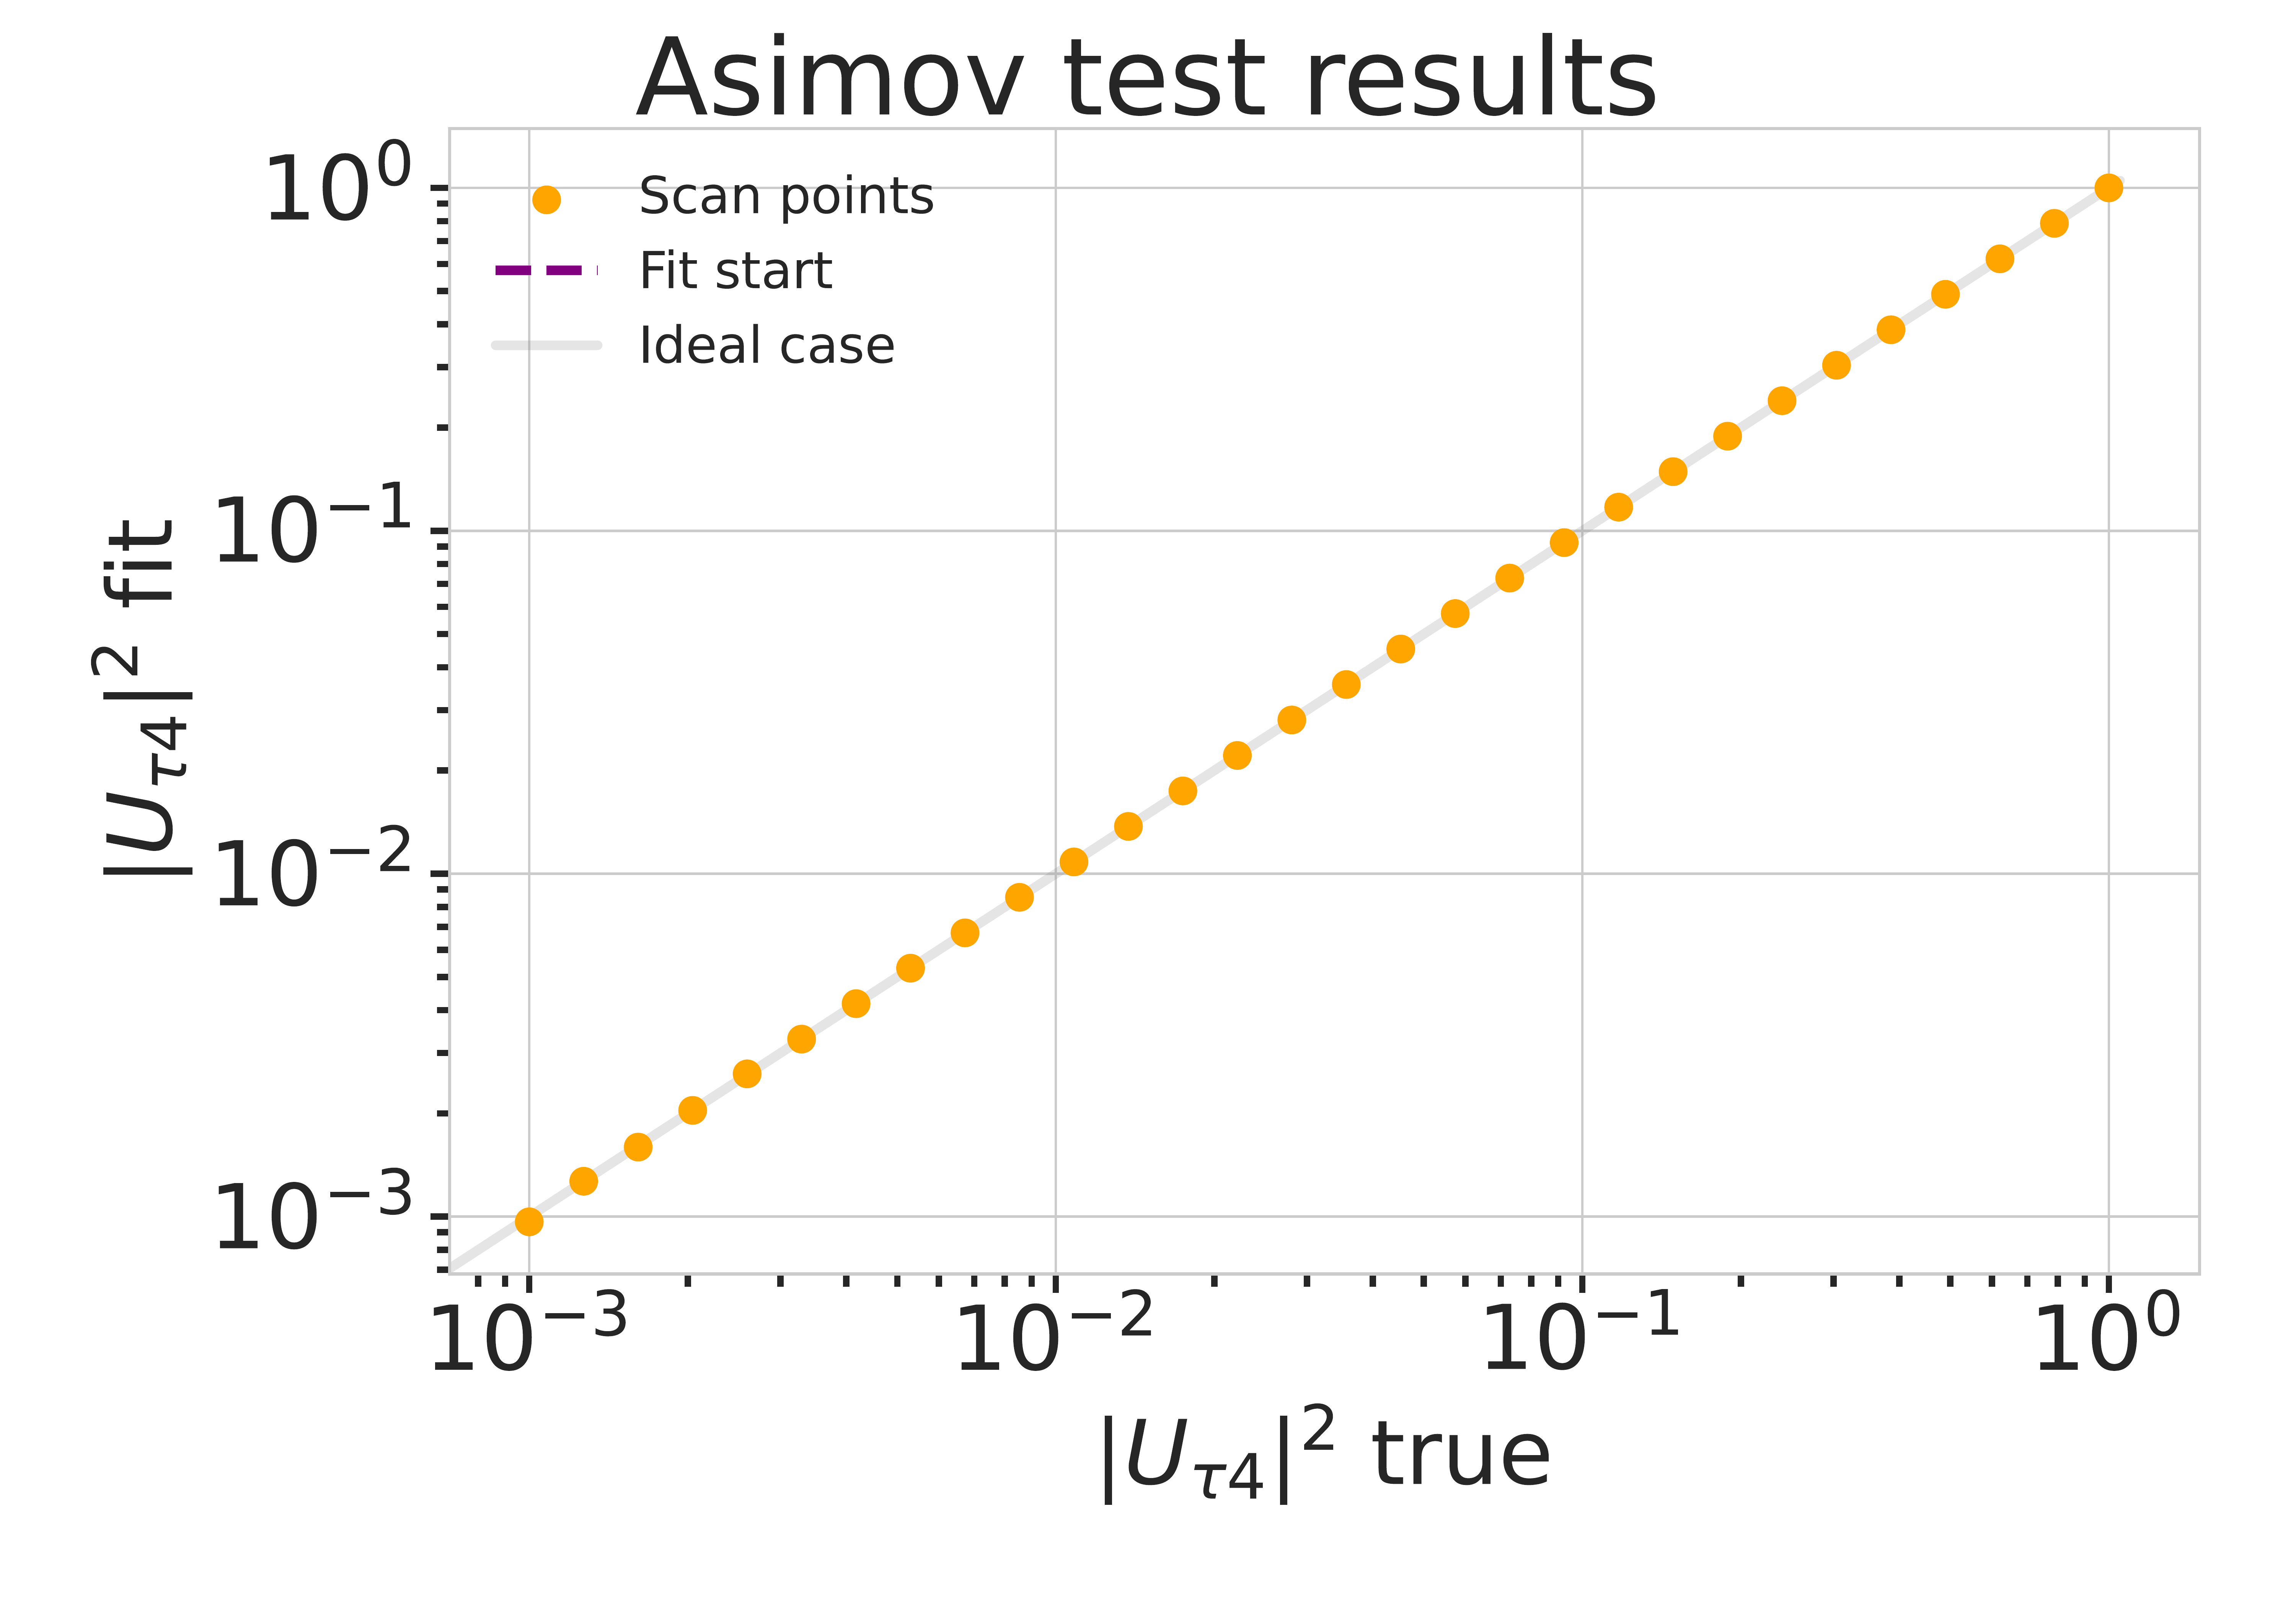
\includegraphics{figures/results/checks/asimov_scan_0.6_GeV-01.png}
	\caption[Asimov inject/recover test (\SI{0.6}{\gev})]{Asimov inject/recover test for the \SI{0.6}{\gev} mass set. Mixing values between $10^{-3}$ and $10^{0}$ are injected and fit back with the full analysis chain. The injected parameter is always recovered within the statistical uncertainty.}
    \labfig{asimov_inject_recover_0.6_GeV}
\end{figure}


% \subsection{Sensitivity}

% \begin{figure}[h]
%     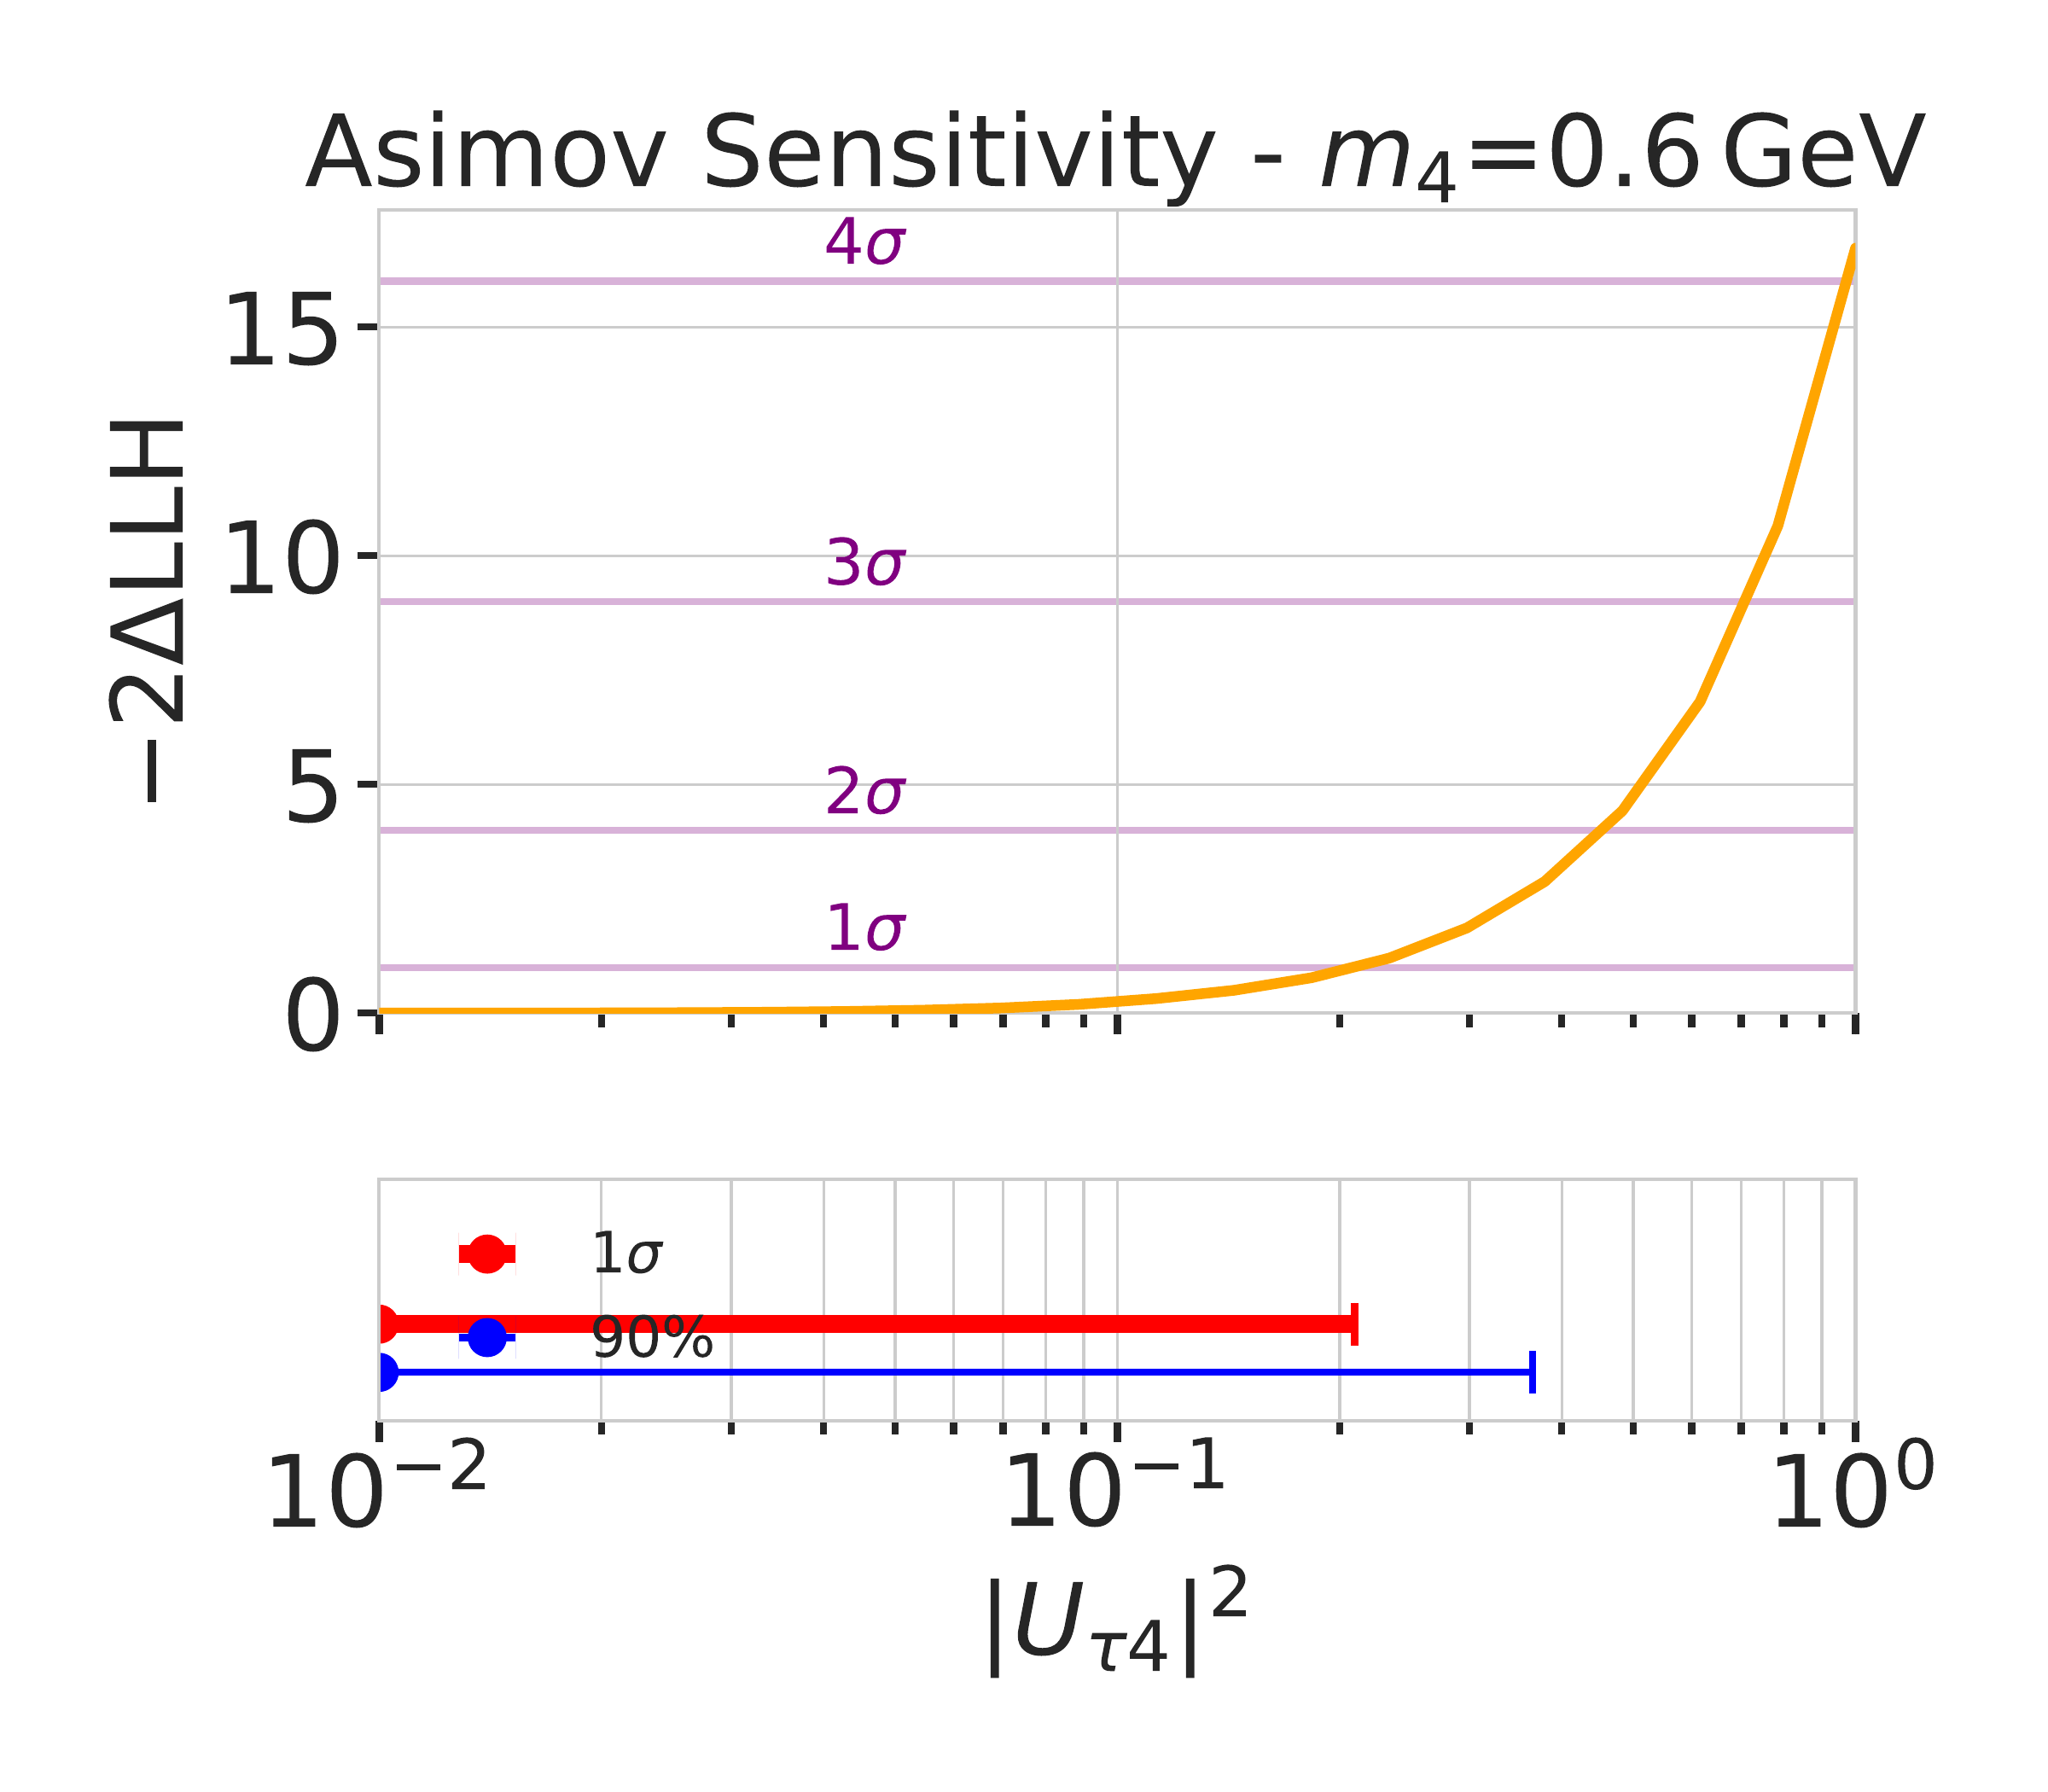
\includegraphics{figures/results/checks/sensitivity_scan_0.6_GeV-1.png}
% 	\caption[Sensitivity scan (\SI{0.6}{\gev})]{Sensitivity scan for the \SI{0.6}{\gev} mass set.}
%     \labfig{sensitivity_scan_0.6_GeV}
% \end{figure}


\subsection{Ensemble Tests} \labsec{pseudo_data_ensemble}

To estimate the goodness of fit, pseudo-data is generated from the MC by injecting the BFP parameters as true parameters and then fluctuating the expected bin counts using Poisson fluctuation. The resulting pseudo-data sets are then fit back with the analysis chain. By comparing the distribution of TS values from this \textit{ensemble} of pseudo-data trials to the TS of the fit to real data, a p-value can be calculated. The p-value is the probability of finding a TS value at least as large as the one from the data fit. \reffig{pseudo_data_ensemble_0.6_GeV}\todo{Add bin-wise TS distribution? Add 3D TS maps?} shows the TS distribution from the ensemble tests for the \SI{0.6}{\gev} mass set and the observed TS value from the fit, resulting in a p-value of \SI{28.5}{\percent}\sidenote{The p-values for the \SI{0.3}{\gev} and \SI{1.0}{\gev} are \SI{28.3}{\percent} and \SI{26.0}{\percent}, respectively.}. Plots for the addition two mass sets are shown in \refsec{pseudo_data_ensemble_appendix}.

\begin{figure}[h]
    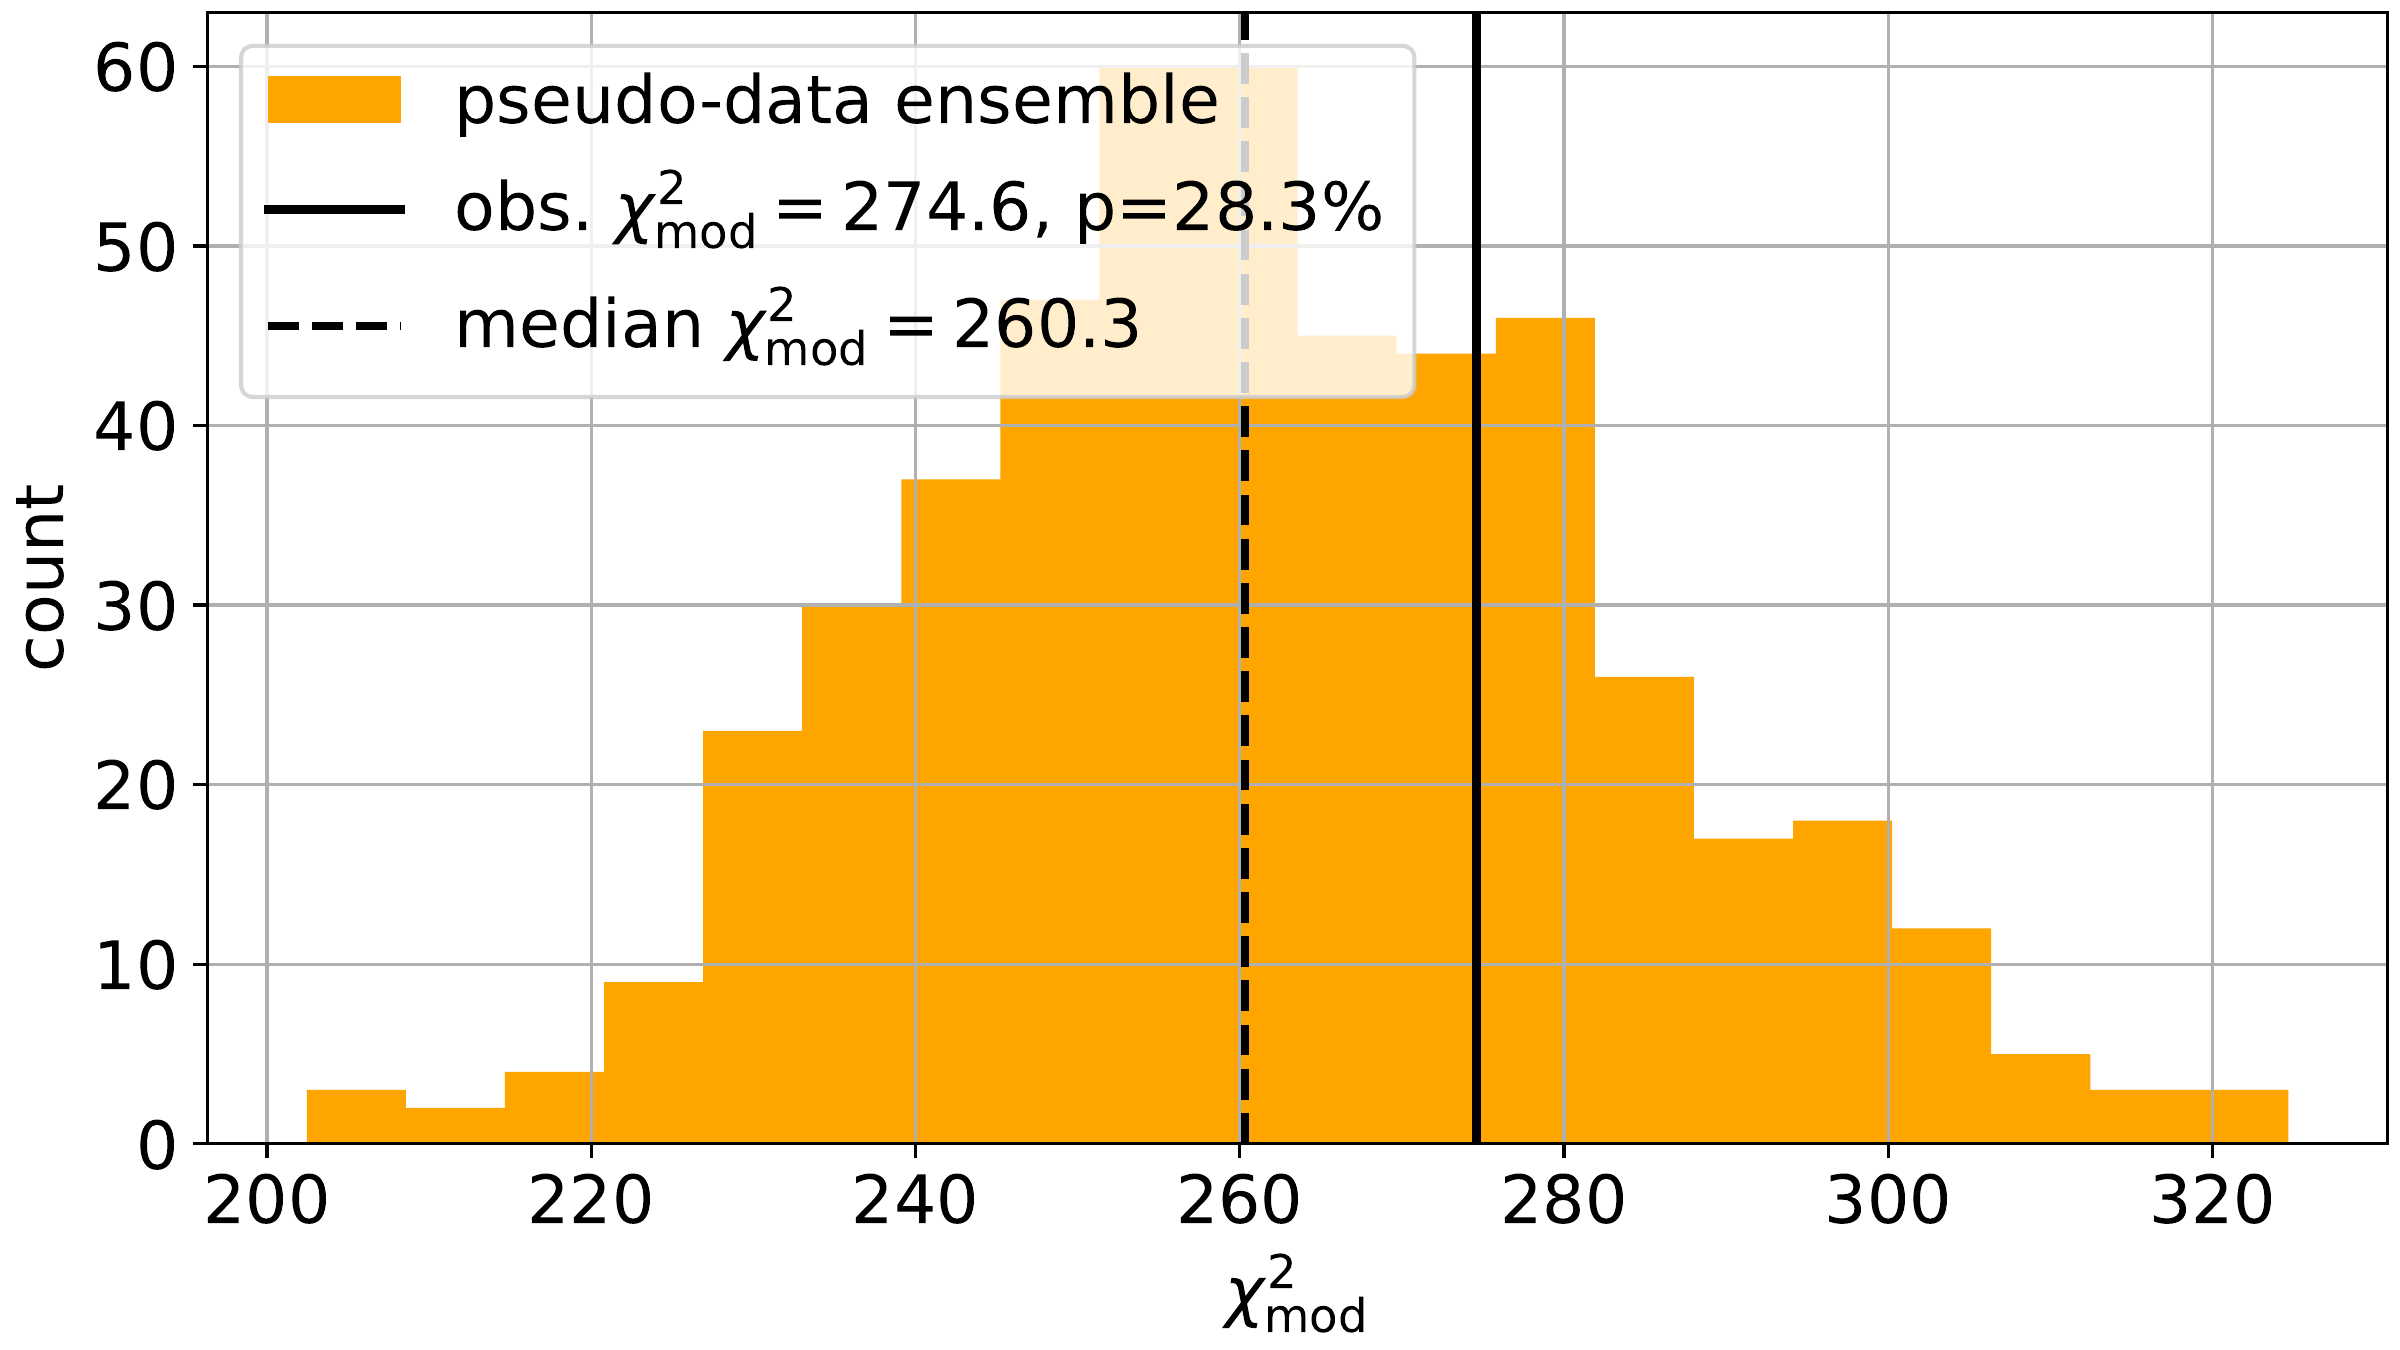
\includegraphics{figures/results/blind_fits/full_blind_fit_0.3_GeV_gauss_plus_poisson_step_3_4-1.png}
	\caption[Pseudo-data trials TS distribution (\SI{0.6}{\gev})]{Observed fit TS and TS distribution from pseudo-data trials for the \SI{0.6}{\gev} mass set.}
    \labfig{pseudo_data_ensemble_0.6_GeV}
\end{figure}


\section{Results}

\todo{Add table with BFP mixings and their uncertainties from scan assuming wilks?}


\subsection{Best Fit Parameters}

\begin{figure*}[h]
    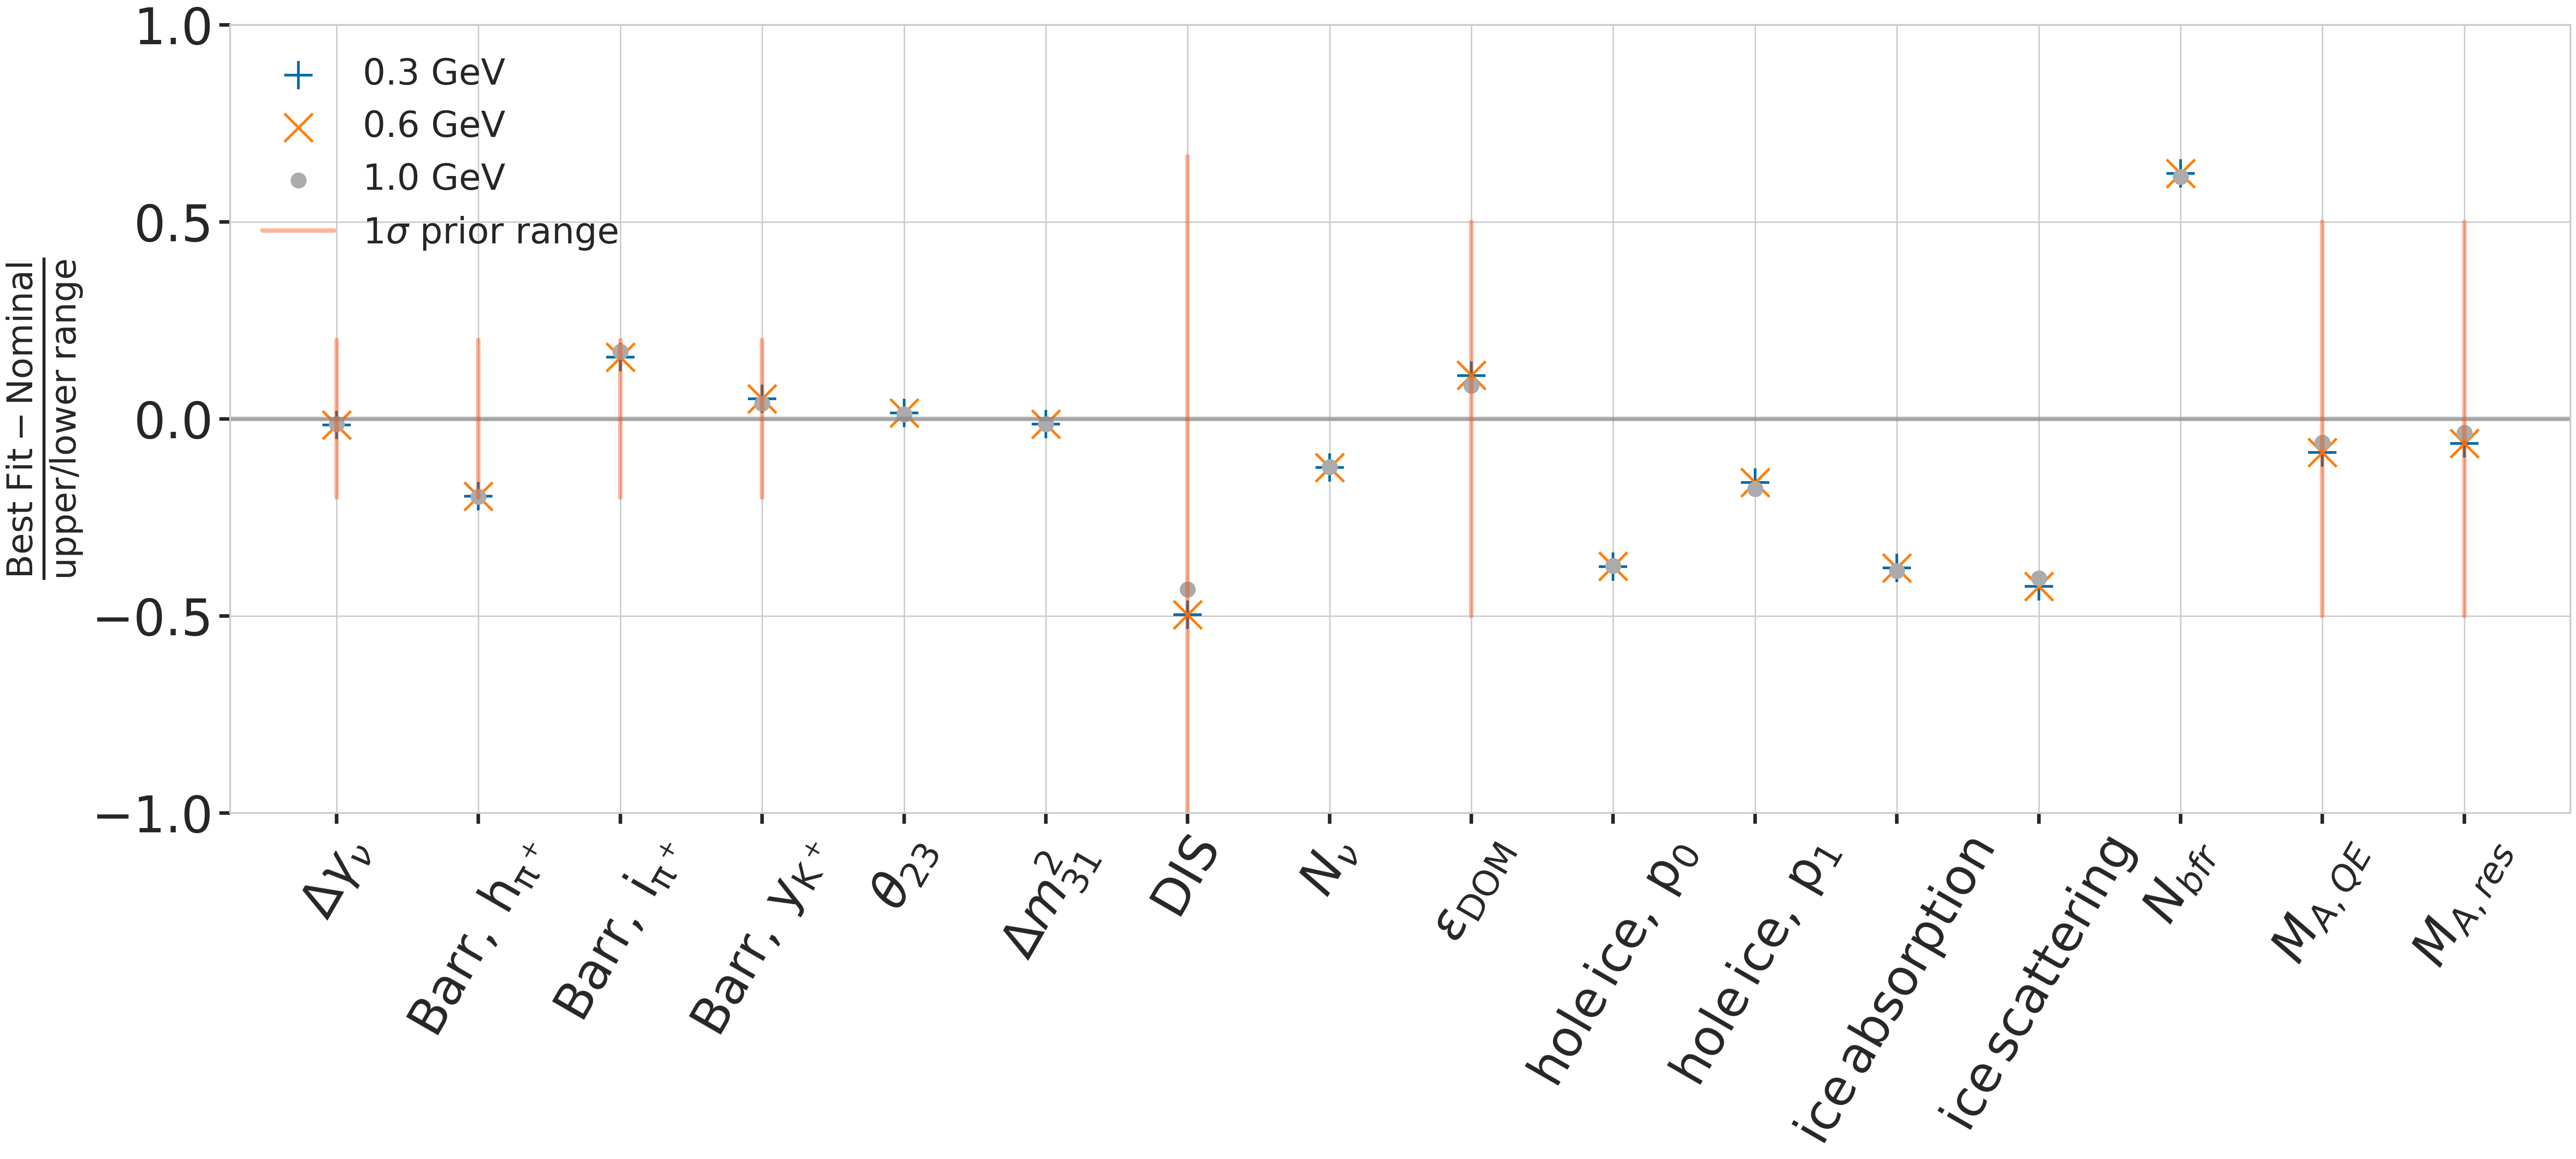
\includegraphics{figures/results/best_fit/hnl_analysis_best_fit_deltas_normed_dist_to_nominal.png}
	\caption[xx]{xx}
    \labfig{best_fit_deltas_normed}
\end{figure*}


\begin{table*}
    \begin{tabular}{ ll lll lll }
    \hline\hline
    \textbf{Parameter} & \textbf{Nominal} & \multicolumn{3}{c}{\textbf{Best Fit}} & \multicolumn{3}{c}{\textbf{Nominal - Best Fit}} \\ 
    & & \textbf{0.3 GeV} & \textbf{0.6 GeV} &  \textbf{1.0 GeV} & \textbf{0.3 GeV} & \textbf{0.6 GeV} &  \textbf{1.0 GeV} \\ 
    \hline\hline
    $\Delta \gamma_\nu$ & 0.000000  & $-$0.007927 & $-$0.007957 & $-$0.006622 & 0.007927  & 0.007957  & 0.006622  \\
    $\rm{Barr} \; h_{\pi^+}$ & 0.000000  & $-$0.147462 & $-$0.147422 & $-$0.148043 & 0.147462  & 0.147422  & 0.148043  \\
    $\rm{Barr} \; i_{\pi^+}$ & 0.000000  & 0.475480  & 0.475323  & 0.520716  & $-$0.475480 & $-$0.475323 & $-$0.520716 \\
    $\rm{Barr} \; y_{K^+}$ & 0.000000  & 0.076161  & 0.076259  & 0.057927  & $-$0.076161 & $-$0.076259 & $-$0.057927 \\
    $\theta_{23} [\si{\degree}]$ & 47.504700 & 48.117259 & 48.118713 & 48.013150 & $-$0.612559 & $-$0.614013 & $-$0.508450 \\
    $\Delta m^{2}_{31} [\si{\electronvolt^2}]$ & 0.002475  & 0.002454  & 0.002454  & 0.002455  & 0.000020  & 0.000020  & 0.000019  \\
    $\rm{DIS}$ & 0.000000  & $-$0.248768 & $-$0.248845 & $-$0.216247 & 0.248768  & 0.248845  & 0.216247  \\
    $N_{\nu}$ & 1.000000  & 0.889145  & 0.889127  & 0.889543  & 0.110855  & 0.110873  & 0.110457  \\
    $|U_{\tau 4}|^2$ & 0.000000  & 0.003017  & 0.000169  & 0.104056  & $-$0.003017 & $-$0.000169 & $-$0.104056 \\
    $\epsilon_{\rm{DOM}}$ & 1.000000  & 1.021987  & 1.022017  & 1.016791  & $-$0.021987 & $-$0.022017 & $-$0.016791 \\
    $\rm{hole \, ice} \; p_0$ & 0.101569  & $-$0.161352 & $-$0.161260 & $-$0.160133 & 0.262921  & 0.262829  & 0.261702  \\
    $\rm{hole \, ice} \; p_1$ & $-$0.049344 & $-$0.073700 & $-$0.073682 & $-$0.076212 & 0.024356  & 0.024338  & 0.026868  \\
    $\rm{ice \, absorption}$ & 1.000000  & 0.943262  & 0.943271  & 0.942023  & 0.056738  & 0.056729  & 0.057977  \\
    $\rm{ice \, scattering}$ & 1.050000  & 0.986150  & 0.986131  & 0.989374  & 0.063850  & 0.063869  & 0.060626  \\
    $N_\rm{bfr}$ & 0.000000  & 0.746674  & 0.746852  & 0.736461  & $-$0.746674 & $-$0.746852 & $-$0.736461 \\
    $M_\rm{A,QE}$ & 0.000000  & $-$0.170430 & $-$0.170677 & $-$0.121335 & 0.170430  & 0.170677  & 0.121335  \\
    $M_\rm{A,res}$ & 0.000000  & $-$0.125908 & $-$0.126076 & $-$0.071727 & 0.125908  & 0.126076  & 0.071727 \\
    \hline
    \end{tabular}
\caption[xx]{xx}
\labtab{best_fit_parameters}
\end{table*}

\subsection{Upper Limits}

\subsection{Post$-$Fit Data/MC Agreement}

\subsection{Likelihood Coverage}
